% ============================================
%  Article Class (This is a LaTeX2e document)
% ============================================
\documentclass[12pt]{scrartcl}
\usepackage[english]{babel}
\usepackage[round]{natbib}
\usepackage[T1]{fontenc}
\usepackage{color}

% ============================
%  Figures and relative paths
% ============================
\usepackage{graphicx}
\graphicspath{{figures/}}

% =======================
%  References to classes
% =======================
\usepackage[colorlinks=true]{hyperref}
% metabolism
\newcommand{\rbametabolism}{\hyperref[sec:rba_metabolism]{\textbf{RBAMetabolism}}}
\newcommand{\compartment}{\hyperref[sec:compartment]{\textbf{Compartment}}}
\newcommand{\species}{\hyperref[sec:species]{\textbf{Species}}}
\newcommand{\reaction}{\hyperref[sec:reaction]{\textbf{Reaction}}}
\newcommand{\speciesreference}{\hyperref[sec:species_reference]{\textbf{SpeciesReference}}}
% parameters
\newcommand{\rbaparameters}{\hyperref[sec:rba_parameters]{\textbf{RBAParameters}}}
\newcommand{\targetdensity}{\hyperref[sec:target_density]{\textbf{TargetDensity}}}
\newcommand{\targetvalue}{\hyperref[sec:target_value]{\textbf{TargetValue}}}
\newcommand{\function}{\hyperref[sec:function]{\textbf{Function}}}
\newcommand{\parameter}{\hyperref[sec:parameter]{\textbf{Parameter}}}
\newcommand{\aggregate}{\hyperref[sec:aggregate]{\textbf{Aggregate}}}
\newcommand{\functionreference}{\hyperref[sec:function_reference]{\textbf{FunctionReference}}}
%macromolecules
\newcommand{\rbamacromolecules}{\hyperref[sec:rba_macromolecules]{\textbf{RBAMacromolecules}}}
\newcommand{\component}{\hyperref[sec:component]{\textbf{Component}}}
\newcommand{\macromolecule}{\hyperref[sec:macromolecule]{\textbf{Macromolecule}}}
\newcommand{\componentreference}{\hyperref[sec:component_reference]{\textbf{ComponentReference}}}
% processes
\newcommand{\rbaprocesses}{\hyperref[sec:rba_processes]{\textbf{RBAProcesses}}}
\newcommand{\process}{\hyperref[sec:process]{\textbf{Process}}}
\newcommand{\machinery}{\hyperref[sec:machinery]{\textbf{Machinery}}}
\newcommand{\machinerycomposition}{\hyperref[sec:machinery_composition]{\textbf{MachineryComposition}}}
\newcommand{\operations}{\hyperref[sec:operations]{\textbf{Operations}}}
\newcommand{\operation}{\hyperref[sec:operation]{\textbf{Operation}}}
\newcommand{\componentmap}{\hyperref[sec:component_map]{\textbf{ComponentMap}}}
\newcommand{\constantcost}{\hyperref[sec:constant_cost]{\textbf{ConstantCost}}}
\newcommand{\cost}{\hyperref[sec:cost]{\textbf{Cost}}}
\newcommand{\targets}{\hyperref[sec:targets]{\textbf{Targets}}}
\newcommand{\targetspecies}{\hyperref[sec:target_species]{\textbf{TargetSpecies}}}
\newcommand{\targetreaction}{\hyperref[sec:target_reaction]{\textbf{TargetReaction}}}
% enzymes
\newcommand{\rbaenzymes}{\hyperref[sec:rba_enzymes]{\textbf{RBAenzymes}}}
\newcommand{\enzyme}{\hyperref[sec:enzyme]{\textbf{Enzyme}}}
\newcommand{\enzymeefficiency}{\hyperref[sec:enzyme_efficiency]{\textbf{EnzymeEfficiency}}}



% ==========
%  Document
% ==========
\begin{document}

\title{XML format for RBA models}
\author{S. Fischer, V. Fromion, A. Goelzer}
\date{\today}

\maketitle

\newpage

\tableofcontents

\newpage

\section{Introduction}

In this document we present the XML structures used to define a RBA model.
A complete RBA model is composed of the following files:
\begin{itemize}
  \item metabolism.xml
  (definition of compartments, metabolic species and metabolic reactions).
  \item parameters.xml
  (definition of density constraints and user-defined functions).
  \item proteins.xml (definition of proteins).
  \item rnas.xml (definition of RNAs).
  \item dna.xml (definition of DNA).
  \item enzymes.xml
  (definition of enzymatic machineries catalyzing metabolic reactions).
  \item processes.xml
  (definition of cell processes necessary to growth and maintenance).
\end{itemize}

For every file, we present the nodes that composes the XML structure.
For every node, we show a class diagram that shows the node's attributes
and the children node that it may/must contain.
We provide a brief description about the relevance of the node
in the RBA model.


\section{Conventions}

\subsection{Naming conventions}

\subsection{Boolean attributes}


\section{metabolism.xml}

\subsection{RBAMetabolism container}

The metabolism file is strongly inspired by SBML.\@
More precisely, it is a subpart of an SBML file.

\subsubsection{RBAMetabolism}
\label{sec:rba_metabolism}

The outermost portion of the metabolism file is an instance of class
\rbametabolism, shown in Figure~\ref{fig:metabolism_doc}.

\begin{figure}
  \centering
  \includegraphics[scale=0.9]{figures/metabolism_doc}
  \caption{XML structure of metabolism document.}
\label{fig:metabolism_doc}
\end{figure}

Currently, \rbametabolism{} has no simple attributes.
It includes exactly one instance of \textbf{ListOf} container classes.
All \textbf{ListOf} classes do not have own attributes,
they are merely used to organize a list of instances from another class.
This organization was inspired by SBML.\@

\subsubsection{Compartment}
\label{sec:compartment}

The \compartment{} class is used to list existing cell compartments.

\paragraph{The \textit{id} attribute}
The \textbf{id} attribute is a string defining the identifier of a compartment.

\subsubsection{Species}
\label{sec:species}

The \species{} class is used to list \emph{metabolic} species.

\paragraph{The \textit{id} attribute}
The \textbf{id} attribute is a string defining the identifier of a metabolite.

\paragraph{The \textit{boundaryCondition} attribute}
The \textbf{boundaryCondition} attribute is a boolean.
If the attribute is set to true, the metabolite is considered to be at
a constant concentration.
In other words, it is not affected by reactions.
This is typical for metabolites in the external medium.


\section{parameters.xml}

\subsection{RBAMetabolism container}

The metabolism file is strongly inspired by SBML.\@
More precisely, it is a subpart of an SBML file.

\subsubsection{RBAMetabolism}
\label{sec:rba_metabolism}

The outermost portion of the metabolism file is an instance of class
\rbametabolism, shown in Figure~\ref{fig:metabolism_doc}.

\begin{figure}
  \centering
  \includegraphics[scale=0.9]{figures/metabolism_doc}
  \caption{XML structure of metabolism document.}
\label{fig:metabolism_doc}
\end{figure}

Currently, \rbametabolism{} has no simple attributes.
It includes exactly one instance of \textbf{ListOf} container classes.
All \textbf{ListOf} classes do not have own attributes,
they are merely used to organize a list of instances from another class.
This organization was inspired by SBML.\@

\subsubsection{Compartment}
\label{sec:compartment}

The \compartment{} class is used to list existing cell compartments.

\paragraph{The \textit{id} attribute}
The \textbf{id} attribute is a string defining the identifier of a compartment.

\subsubsection{Species}
\label{sec:species}

The \species{} class is used to list \emph{metabolic} species.

\paragraph{The \textit{id} attribute}
The \textbf{id} attribute is a string defining the identifier of a metabolite.

\paragraph{The \textit{boundaryCondition} attribute}
The \textbf{boundaryCondition} attribute is a boolean.
If the attribute is set to true, the metabolite is considered to be at
a constant concentration.
In other words, it is not affected by reactions.
This is typical for metabolites in the external medium.


\section{proteins.xml, rnas.xml and dna.xml}

All these files use instances of the class \rbamacromolecules.


\subsection{RBAMacromolecules}
\label{sec:rba_macromolecules}

The outermost portion of the metabolism file is an instance of class
\rbamacromolecules, shown in Figure~\ref{fig:macromolecules}.

\begin{figure}
  \centering
  \includegraphics[scale=0.8]{figures/macromolecules}
  \caption{XML structure of macromolecule document.}
\label{fig:macromolecules}
\end{figure}

\rbamacromolecules{} has no simple attributes.
It contains exactly one instance of \textbf{ListOfComponents}
and \textbf{ListOfMacromolecules}.


\subsection{Component}
\label{sec:component}

The \component{} class is used to define the components of a \macromolecule{}
(Fig.~\ref{fig:macromolecules}).
For example, these are expected to be amino acids, vitamins and ions for
proteins.
Note that they use separate identifiers as metabolic \species.
\componentmap{}s define how they are assembled from metabolites.


\paragraph{The \textit{id} attribute}
The \textbf{id} attribute is a string defining the identifier of a component.

\paragraph{The \textit{weight} attribute}
The \textbf{weight} attribute is a real number defining the weight of a
component.
This information is essential for the density constraints.
The weight of a macromolecule is defined as the sum of the weight of its
components.
Note that units used for the weight constraint must be consistent across
files.

\paragraph{The \textit{name} and \textit{type} attributes}
The \textbf{name} and \textbf{type} attributes are string that provide
additional information about the component.
The name is a standard name of the component
(\textit{e.g.} full amino acid name).
The type can be used to distinguish components if necessary
(\textit{e.g.} in amino acids, vitamins, ions).


\subsection{Macromolecule}
\label{sec:macromolecule}

The \macromolecule{} class is used to define macromolecular species
(Fig.~\ref{fig:macromolecules}).
Its composition is given by a \textbf{ListOfComponentReferences}.

\paragraph{The \textit{id} attribute}
The \textbf{id} attribute is a string defining the identifier of
the macromolecule.

\paragraph{The \textit{compartment} attribute}
The \textbf{compartment} attribute must match the identifier of a \compartment.
It represents the compartment where the molecule is thought to be active.


\subsection{ComponentReference}
\label{sec:component_reference}

The \componentreference{} class is used to refer to a \component{}
and associate with it a stoichiometry (Fig.~\ref{fig:macromolecules}).

\paragraph{The \textit{component} attribute}
The \textbf{component} attribute must match the identifier of a \component{}
defined in the same \rbamacromolecules{} instance.

\paragraph{The \textit{stoichiometry} attribute}
The \textbf{stoichiometry} is a positive real number.
It repensents the stoichiometry of a \component{} in a given context
(typically the composition of a \macromolecule).


\section{processes.xml}

\subsection{Rationale}

The process file is used to define cellular processes involved in
the production or degradation of macromolecules.
In proteins.xml, rnas.xml and dna.xml, we have described proteins in terms of
components (amino acid residues, nucteotides, protein cofactors).
processes.xml defines how components are assembled from metabolites and
what machines are needed to catalyze the assembly.

A typical example of a cellular process is protein translation.
Translation relies on ribosomes as a molecular machine,
and participates in protein production.
The metabolites used during proteins assembly include
charged and uncharged-tRNAs and GTP/GDP,
e.g.\ an alanine residue is obtained by using a charged tRNA-alanine and GTP as
reactants, generating an uncharged tRNA, GDP and water as a byproduct.

Theoretically, the translation of a protein could be written down as a single reaction,
listing all charged-/uncharged-tRNAs, GTP/GDP, according to the SBML format.
In a model containing 1000 proteins, we would have to write 1000 reactions
that follow the same template.
Now, if we add other processes undergone by proteins
(translation, chaperoning, translocation),
we would have to add more reactions per protein to account for the fact that each
process is catalyzed by the appropriate molecular machine such as an enzyme or a ribosome.
For example, if all proteins need chaperones for folding,
we need to add 1000 reactions for chaperoning to the pre-existing
1000 reactions for reaction synthesis.
If we add translocation/transport of proteins to target locations,
that's 1000 more reactions.
If we update the template of one of the process,
e.g. we revise the number of GTPs that are consumed per amino acid for protein synthesis,
we need to rewrite all 1000 reactions describing protein synthesis,
which is an extremely error-prone process.

RBA \process{}es can be seen as template reactions that specify how
\macromolecule{}s are produced and degraded based on their \component{}s.
Instead of writing one reaction per protein,
we write one generic reaction per process,
and proteins are seen as input of these processes.
Every cellular process is described by
(1) the molecular machine that catalyzes the process (e.g.\ the ribosome),
(2) the list of macromolecules to be processed or produced (e.g.\ proteins),
(3) the processing costs (e.g.\ tRNAs and GTP consumed to assemble an amino acid), and
(4) the efficiency of the molecular machine in catalyzing the process,
which corresponds to the rate of the process per amount of process machinery
(e.g.\ translation rate for ribosomes).

The processing costs are defined by a \processingmap{},
which explicits how every \component{} is processed, i.e.
what \species{} are consumed and what \species{} are
produced as byproducts of the assembly process.
For example, in order to assemble an Alanine residue,
a charged alanine-tRNA is consumed along with GTP,
and an uncharged alanine-tRNA and GDP are generated as byproducts.
\processingmap{}s define one reaction per \component(), frow which
the overall production/degradation reactions of \macromolecule{}s can be deduced.

Processes are flexible:
\macromolecule{}s can be listed as input of several processes.
For example, proteins may undergo translation, folding and translocation.
The overall production/degradation reaction of a \macromolecule{} reflects
all the \process{}es it traverses.
When we modify a process,
e.g.\ we update the number of GTPs consumed per amino acid,
it automatically affects the production of all input macromolecules.


[FIGURE AVEC EXEMPLE?]

\subsection{RBAProcesses}
\label{sec:rba_processes}

The outermost part of the process file is an instance of class
\rbaprocesses, shown in Figure~\ref{fig:processes_doc}.

\begin{figure}
  \centering
  \includegraphics[scale=0.8]{figures/processes_doc}
  \caption{XML structure of process document.}
\label{fig:processes_doc}
\end{figure}

\rbaprocesses{} has no simple attributes.
It contains exactly one instance of \textbf{ListOfProcesses}
and \textbf{ListOfProcessingMaps}.


\subsection{Process}
\label{sec:process}

The \process{} class is used to define cellular processes
(Fig.~\ref{fig:processes_process}).

\begin{figure}
  \centering
  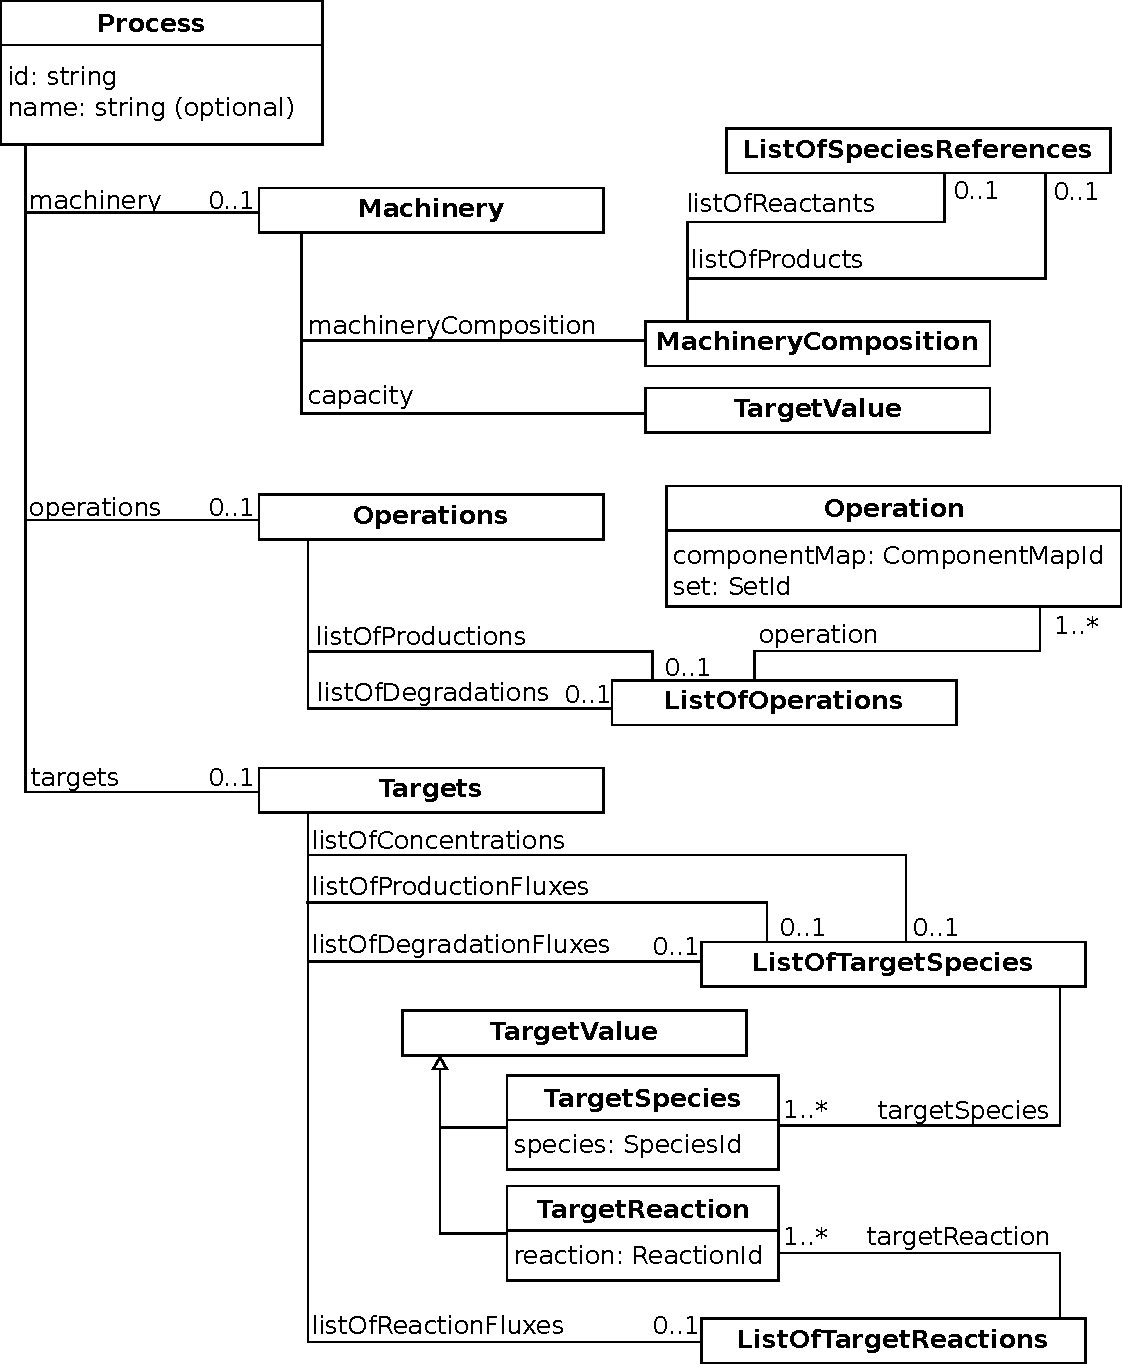
\includegraphics[scale=0.8]{figures/processes_process}
  \caption{Class used to store processes.}
\label{fig:processes_process}
\end{figure}

A \process{} revolves around 2 optional substructures.
The \machinery{} is the molecular entity enabling the process
(\textit{e.g.} ribosome for translation.)
Each machinery unit has a limited production/degradation capacity.
Every macromolecule produced by a process has a metabolite cost
(metabolites needed to produce/degrade it and byproducts).
However, if a machinery is defined, there is an additional cost
to produce the machinery that will enable the production/degradation of the
target.
This is similar to the production of \enzyme{}s in order to catalyze
metabolic \reaction{}s.

\processings{} define the sets of macromolecules that a process
produces or degrades.
The production reaction of a \macromolecule{} is determined by the \process{}es
it goes through.
For example, a protein's production reaction is defined by listing
the protein as an input in the \processings{} of the translation process.
If a protein is not listed as an input of any process, its production reaction
is empty, meaning that it does not cost anything to produce the protein.
\processings{} break down \macromolecule{}s in metabolic \species{}
and \machinery{} costs.

\paragraph{The \textit{id} attribute}
The \textbf{id} attribute is a string defining the identifier of a process.

\paragraph{The \textit{name} attribute}
The \textbf{name} attribute is a string that can be used to give the process
a more human understandable name.


\subsection{Machinery}
\label{sec:machinery}

The \machinery{} class defines the machinery used by a process
(Fig.~\ref{fig:processes_process}).
\machinery{} has no simple attributes.
If a \machinery{} is defined, it defines a \emph{capacity constraint}.
Every \machinery{} unit is produced accordint to the reaction
defined by a \machinerycomposition.
Every unit also has a capacity defined by a \targetvalue.
The capacity defines how many targets a \machinery{} can process in 1 unit of
time.
Total capacity (base capacity multiplied by number of \machinery{} units)
must always exceed the number of targets produced.


\subsection{MachineryComposition}
\label{sec:machinery_composition}

The \machinerycomposition{} class defines the assembly of a complex
molecular machinery (Fig.~\ref{fig:processes_process}).
\machinerycomposition{} has no simple attributes.
It contains two \textbf{ListOfSpeciesReferences}.
One is for reactants, the other for potential byproducts of the assembly reaction
of the complex itself (e.g. GDP when connecting ribosomal subunits).
Note that in this case, \speciesreference{}s can refer to \emph{both}
metabolic \species{} and \macromolecule{}s.
The assembly reaction should contain obvious components of the machinery,
but also metabolic costs related to assembly (such as ATP/GTP costs)
\emph{unless} these costs are already covered by a process.


\subsection{Processings}
\label{sec:processings}

The \processings{} relates \macromolecule{}s production/degradation to
some given \process{}es (Fig.~\ref{fig:processes_process}).
\processings{} has no simple attributes.
It may contain two \textbf{ListOfProcessings}, one for production and one for
degradation.


\subsection{Processing}
\label{sec:processing}

The \processing{} class defines how \macromolecule{}s are produced/degraded
(Fig.~\ref{fig:processes_process}).
\processing{} is used to break down \macromolecule{}s into metabolites
by linking them to a \processingmap.
It contains one \textbf{ListOfSpeciesReferences} that lists \macromolecule{}s
that are inputs of this process.
In this context, the species of a \speciesreference{} must be a macromolecule
and the stoichiometry attribute is ignored.

\paragraph{The \textit{processingMap} attribute}
The \textbf{processingMap} attribute must match the identifier of a
\processingmap.
This \processingmap{} will be used to compute the production/degradation
reaction of \macromolecule{}s, as well as \machinery{} costs.

\paragraph{The \textit{set} attribute}
The \textbf{set} attribute must refer to a \macromolecule{} set.
Currently, the only acceptable values are \textbf{protein}, \textbf{rna}
and \textbf{dna}.
\macromolecule{}s that are listed as input must belong to this set.


\subsection{ProcessingMap}
\label{sec:processing_map}

The \processingmap{} class is used to convert \macromolecule{}s in
metabolic and machinery costs (Fig.\ref{fig:processes_processing_map}).

\begin{figure}
  \centering
  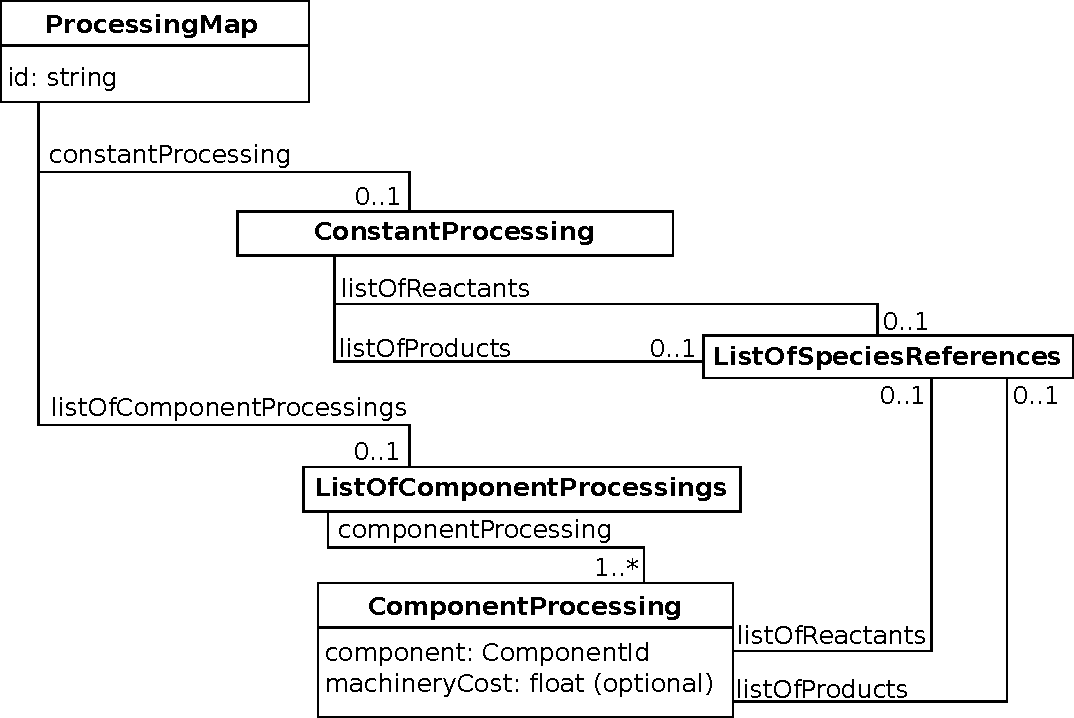
\includegraphics[scale=0.8]{figures/processes_processing_map}
  \caption{Class used to compute production/degradation of macromolecules.}
\label{fig:processes_processing_map}
\end{figure}

There are two types of processings.
The \constantprocessing{} lists metabolites that are always consumed or
produced when processing a macromolecule, no matter its composition
(\textit{e.g.} translation initiation).
The \textbf{ListOfComponentProcessing} container details
\componentprocessing{}s depending on the individual
\component{}s of the \macromolecule{}.
They cover metabolites used to assemble the \component{} onto the nascent
\macromolecule{}.
They also cover machinery costs, \textit{i.e.} how many \machinery{} units
are needed to assemble the \component{}.

\paragraph{The \textit{id} attribute}
The \textbf{id} attribute is a string defining the identifier of a
processing map.


\subsection{ConstantProcessing}
\label{sec:constant_processing}

The \constantprocessing{} class defines metabolites consumed and byproducts
generated by an assembly process (Fig.\ref{fig:processes_processing_map}).
It contains two \textbf{ListOfSpeciesReferences}, one for metabolites
consumed and one for metabolites produced.
Note that in this context, a \speciesreference{} must refer to a
metabolic \species.


\subsection{ComponentProcessing}
\label{sec:component_processing}

The \componentprocessing{} class defines metabolites consumed and byproducts
generated when assembling a specific \component{}
(Fig.\ref{fig:processes_processing_map}).
It contains two \textbf{ListOfSpeciesReferences}, one for metabolites
consumed and one for metabolites produced.
Note that in this context, a \speciesreference{} must refer to a
metabolic \species.
Additionally, it defines a machinery cost used in a \machinery{}'s
capacity constraint.

\paragraph{The \textit{component} attribute}
The \textbf{component} attribute is a string that must match the identifier
of a \component{}.

\paragraph{The \textit{machineryCost} attribute}
The \textbf{machineryCost} attribute is a real value that is used to
compute how many \machinery{} units are needed to assemble the \component{}.
For example, let the machinery cost for the processing of an amino acid be 1.
The capacity of the \machinery{} (the ribosome) is the number of amino acids
it can assemble per unit of time.
The machinery cost allows to compute how many ribosomes are needed
to produce the \component{} and, in the end, the \macromolecule{}
(in this example the number of amino acids divided by the ribosome's capacity).

\subsection{Examples}

The best example to illustrate processes is protein translation
(Fig.~\ref{fig:processes_ex_1}).
The XML structures are quite long, but processes depend on 3 relatively
simple substructures.
First, we define the process machine.
The definition is reminiscent of enzymes:
a machine composition, here all ribosome components (proteins and RNAs),
and a catalytic rate, here expressed in number of amino acids per hour.
Second, we list all macromolecules that undergo the process, here all proteins.
Finally, the processing map, containing one reaction per macromolecule component.
The question this structure answers is the following:
my macromolecule contains a component named "alanine residue",
how do I produce it from metabolites? Is the process machine involved?
The answers are: for every alanine residue, you consume a charged t-RNA,
water and GTP, by-producing an uncharged t-RNA, GDP, phosphate and protons.
The machine cost is an additive cost that is related to the capacity defined earlier.
For translation, we define the machine cost for every amino acid to be 1.
In the end the total production cost of a protein is its number of amino acids.
We defined the ribosome capacity in terms of amino acid per hour, say 1000.
If a protein has 500 amino acids, a single ribosome will be able to produce
two copies of this protein per hour.

The machine costs define a capacity constraint for the cell:
in order to be viable, the cell needs not only to produce essential macrocomponents,
but also the machines that assemble these macrocomponents.
Production of machines cannot be neglected, as they increase very rapidly.
When the production rate of macromolecule increases,
the amount of machines needed for production increases in a seemingly linear fashion.
However, machines are themselves composed of macromolecules (\ref{fig:processes_ex_2}),
and you need more machines to assemble those.
Roughly speaking, if you want more proteins, you need to produce more ribosomes.
But if you want more ribosoms, you need ribosomes to produce the new ribosomes.
In the end the amount of machines increases more than linearly,
imposing strong constraints on the cell.

\begin{figure}
  \centering
  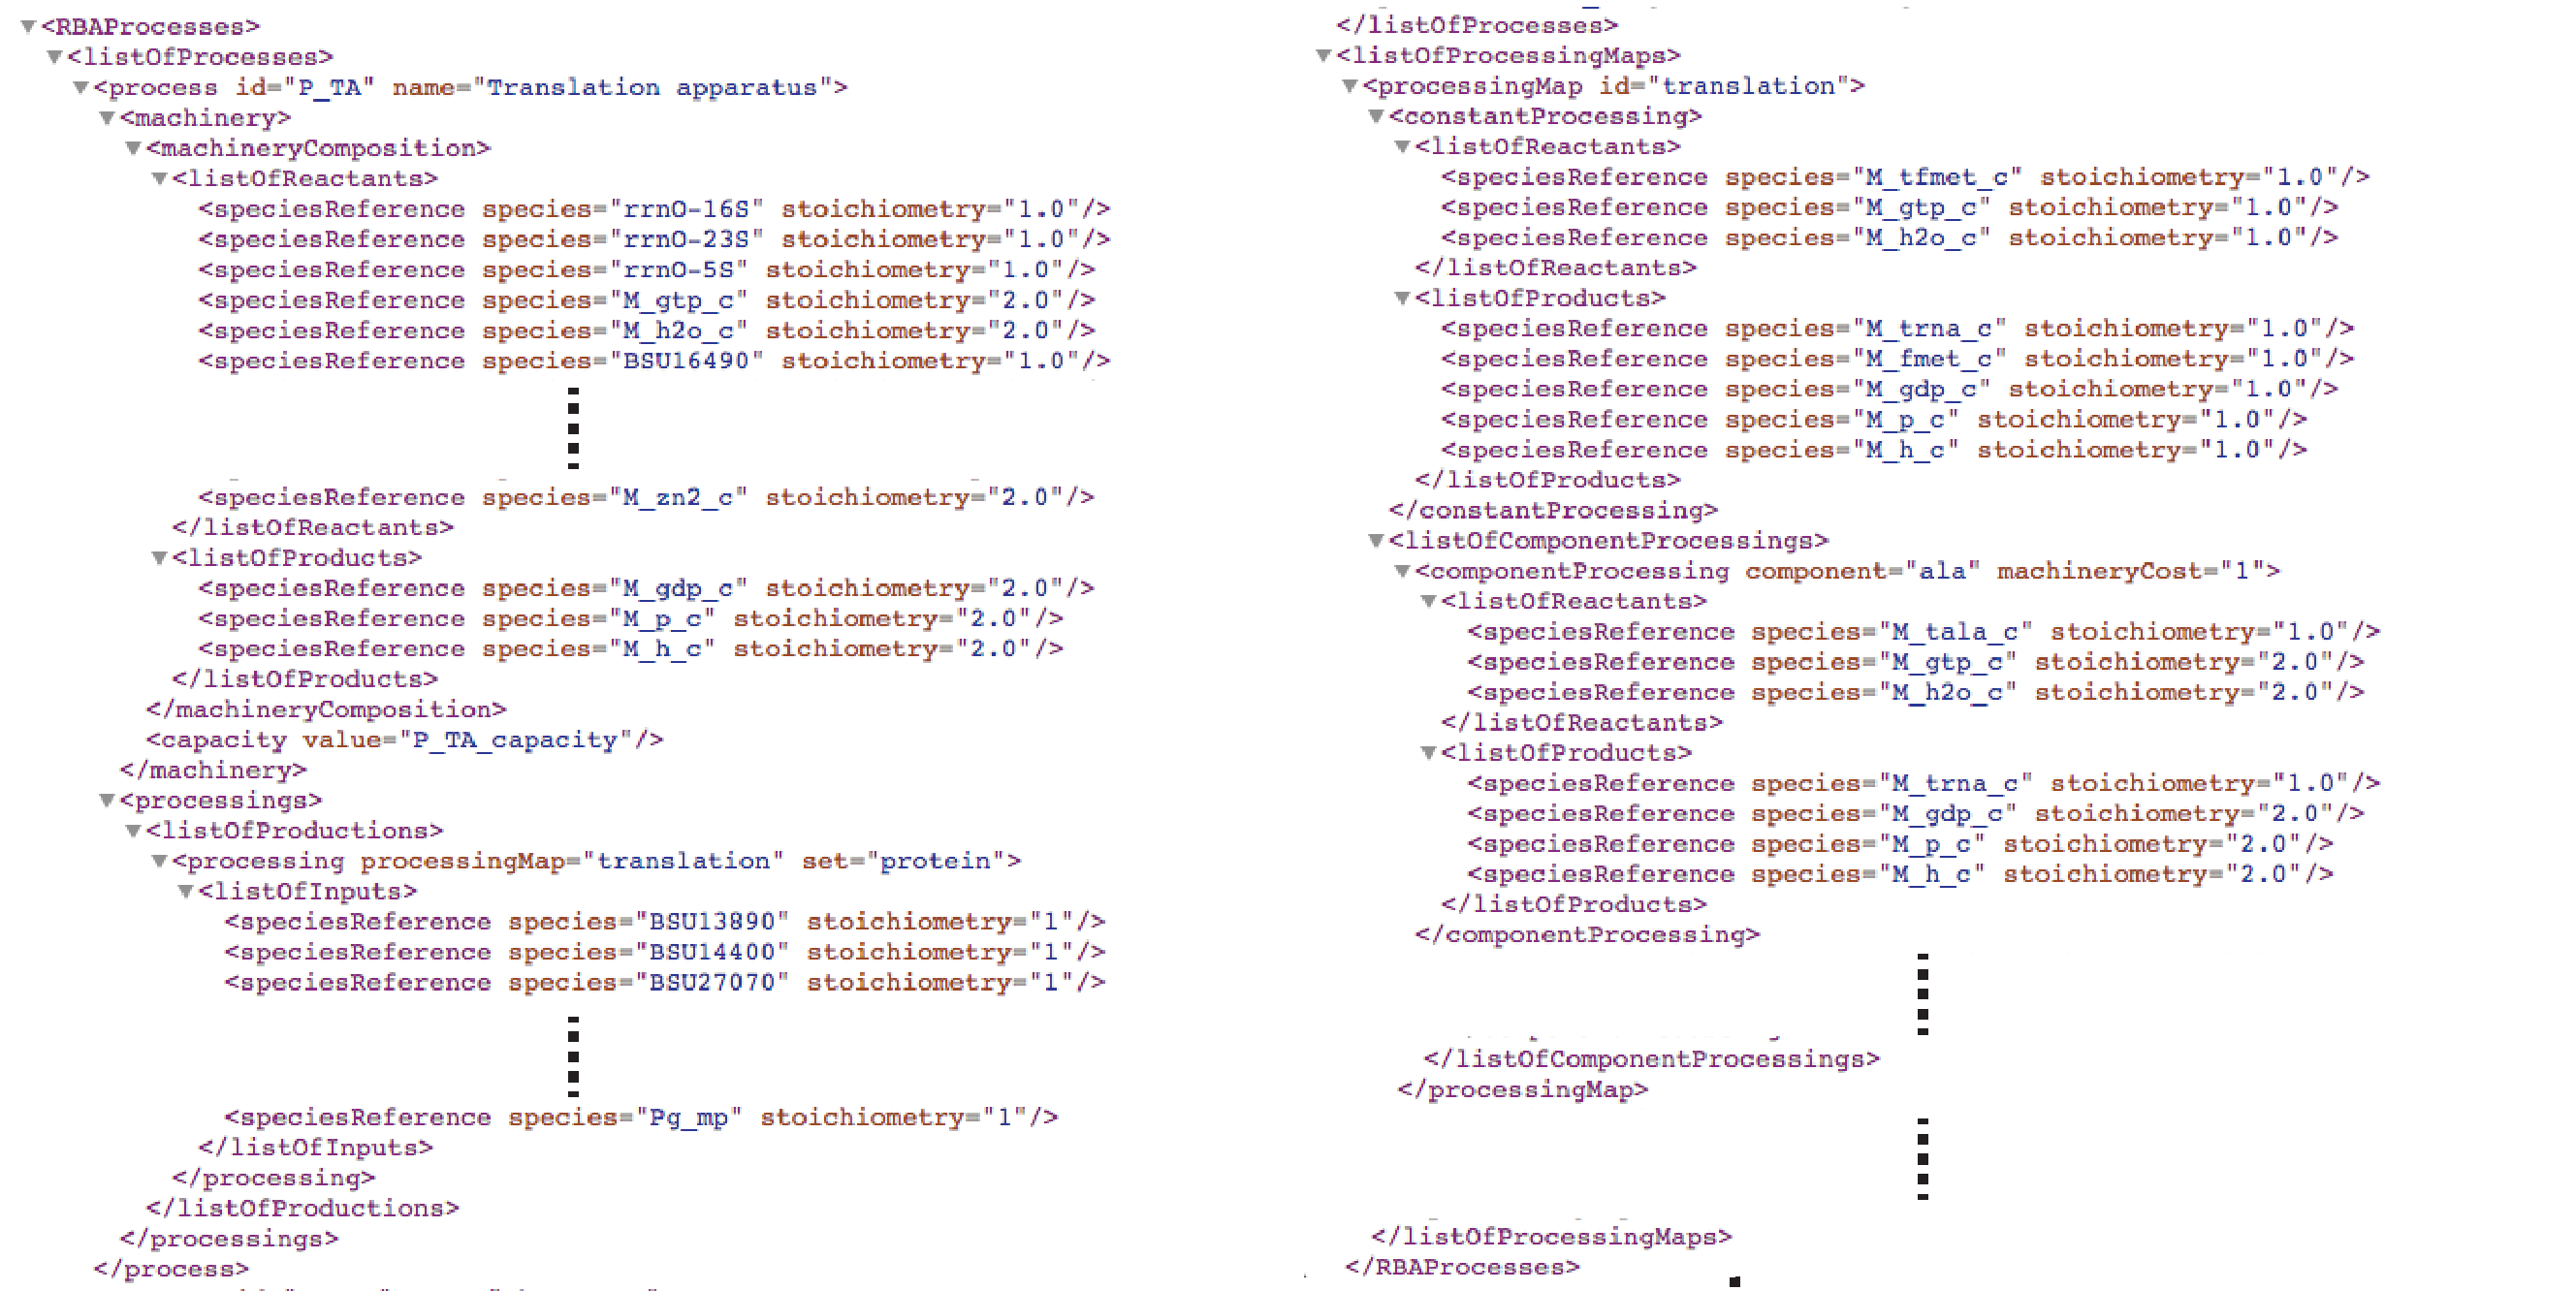
\includegraphics[scale=0.4]{figures/processes_ex_1}
  \caption{processes.xml from the hand curated model for model bacteria \textit{B. subtilis}.
  Large chunks of the files were removed for brevity.
  This example focuses on some aspects of the definition of the translation process.
  The first element that is defined is the process machine: the ribosome.
  The machine is defined as a single assemble reaction from
  macromolecules (ribosomal proteins and rRNAs)
  and metabolites (GTP needed to assemble ribosomal proteins and rRNAs).
  Process machines have a catalytic rate termed capacity:
  for the ribosome, this is the number of amino acids processed per hour,
  later defined by the parameter P\_TA\_capacity.
  Finally the process contains the list of macromolecules to produce or degrade,
  here all the proteins in the model.
  A processing map explicits how macromolecules are produced from their components.
  Here, the processing map starts by defining metabolites that are consumed and
  produced independent of protein composition (translation initiation).
  We also show how an alanine residue is built from metabolites.}
  \label{fig:processes_ex_1}
\end{figure}

\begin{figure}
  \centering
  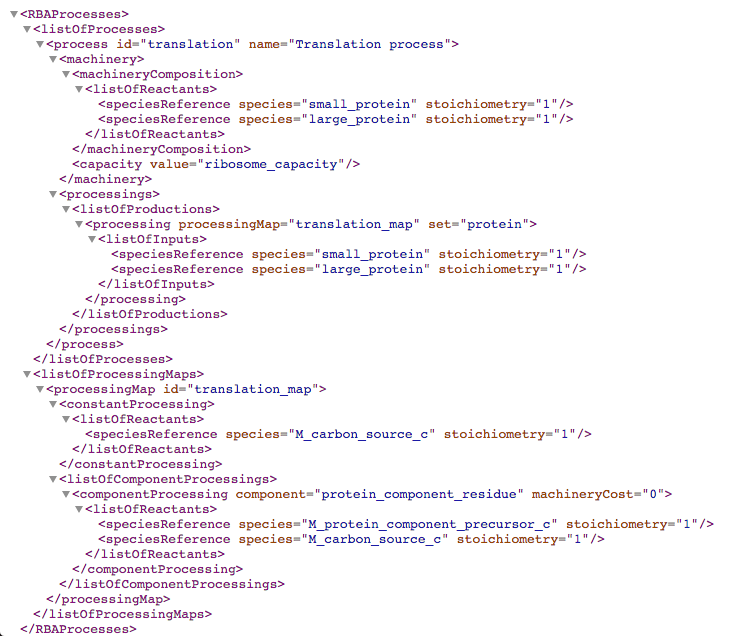
\includegraphics[scale=0.6]{figures/processes_ex_2}
  \caption{processes.xml from the minimal model.
  We only define one process corresponding to pseudo-translation.
  It contains a two-protein machine with a capacity that we will define later.
  We list all the proteins from the model as input of translation.
  Proteins only had one component so the processing map is short.
  We define a constant cost corresponding to translation initiation
  and metabolites consumed for every residue that has to be assembled. }
  \label{fig:processes_ex_2}
\end{figure}


\section{enzymes.xml}

The enzyme file is used to define enzyme composition and their catalytic efficiency.
It defines efficiency constraints in the RBA model.
These constraints ensure that a reaction flux is smaller than
the product of efficiency and concentration of the enzyme catalyzing
the reaction.

\subsection{RBAEnzymes}
\label{sec:rba_enzymes}

The outermost portion of the metabolism file is an instance of class
\rbaenzymes, shown in Figure~\ref{fig:enzymes_doc}.

\begin{figure}
  \centering
  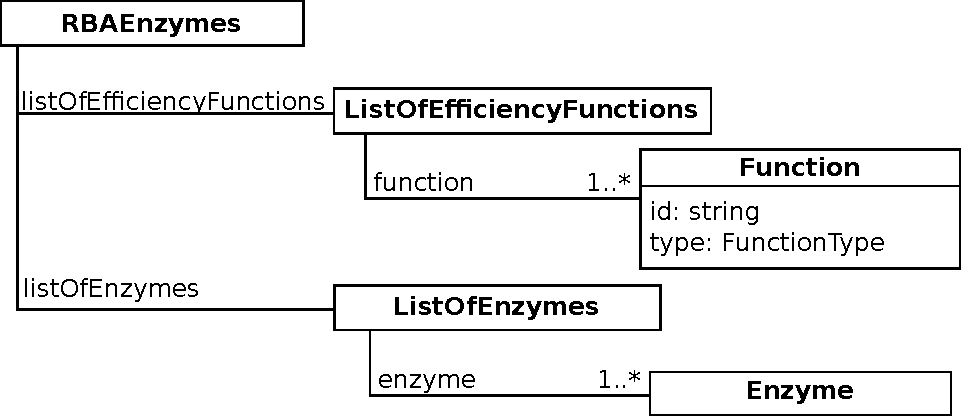
\includegraphics[scale=0.8]{figures/enzymes_doc}
  \caption{XML structure of enzyme document.}
\label{fig:enzymes_doc}
\end{figure}

\rbaenzymes{} has no simple attributes.
It contains excatly one instance of \textbf{ListOfEnzymes} that is used
to store \enzyme{} information.


\subsection{Enzyme}
\label{sec:enzyme}

The \enzyme{} class is used to define enzymes
(Fig.~\ref{fig:enzymes_doc}).

It contains a \machinerycomposition{} that refers to metabolic \species{}
and \macromolecule{}s composing the \enzyme{}.
Note that the composition can be left unspecified.
In this case, the reaction associated with the enzyme is considered spontaneous.

\paragraph{The \textit{id} attribute}
The \textbf{id} attribute is a string defining the identifier of
the enzyme.

\paragraph{The \textit{reaction} attribute}
The \textbf{reaction} attribute must match the identifier of a metabolic
\reaction.
It represents the reaction catalyzed by the enzyme.
This must be a one-to-one mapping.
A \reaction{} can only have one associated \enzyme{}.
If several \enzyme{}s catalyze the same \reaction{},
the \reaction{} must be duplicated.

\paragraph{The \textit{forwardEfficiency} attribute}
The \textbf{forwardEfficiency} attribute must match the identifier of a
parameter (\function{} or \aggregate{}).
It represents the forward catalytic constant.

\paragraph{The \textit{backwardEfficiency} attribute}
The \textbf{backwardEfficiency} attribute must match the identifier of a
parameter (\function{} or \aggregate{}).
It represents the backward catalytic constant
(only applicable if reaction catalyzed by enzyme is reversible).

\paragraph{The \textit{zeroCost} attribute}
The \textbf{zeroCost} attribute is a boolean value.
If set to true, the reaction associated may occur without having to produce
the enzyme.
If set to false or unspecified, an efficiency constraint is created where the
flux through the reaction has to be smaller than the product of enzyme
efficiency and enzyme concentration.



\end{document}
% ----------------------------------------------------------------
